
% \section{Computer Vision}\label{chap2:compvis}


\section{From Pixels to Voxels}\label{chap2:voxels}
Images are the ubiquitous source of information for visual tasks. They are pictures that are stored in electronic form, more specifically, matrices where each cell is called a pixel. Each cell in the matrix has a value: for black and white images this value falls in the range from 0 to 255 and in color images the cell is extended to hold three values instead of one, making it capable of storing the color a representation based on a given color schemes. There are many color schemes but red, green, blue RGB is a widely used and can be combined to represent any color. In other words, RGB images are pictures which are stored electronically as three-dimensional matrices following a given RGB color scheme. 

\begin{figure}[!ht]
        \centering
        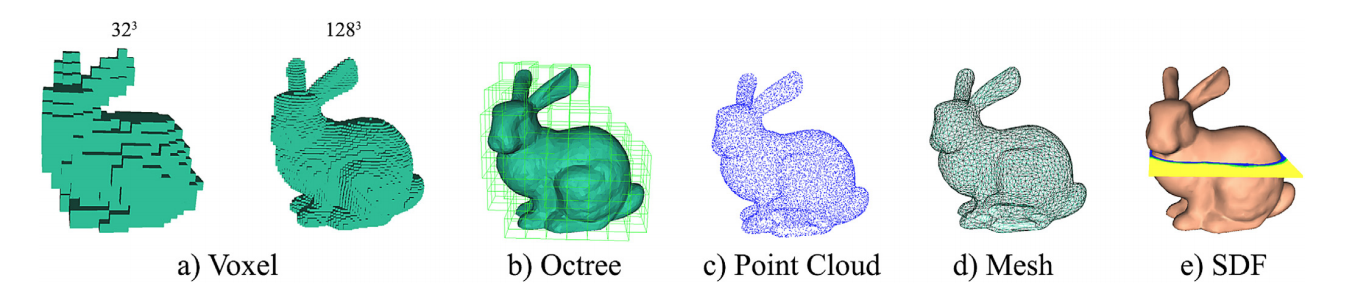
\includegraphics[width=1\textwidth]{images/3drepresentations.png}
        \caption{The Stanford Bunny in different 3D representations                     \cite{fahim2021single}
        .}
        \label{fig:3drepresentations}
\end{figure}

Moreover, RGB-D images contribute to this representation by storing a fourth channel, i.e. a depth map, alongside the 2D color information (RGB). Depth is the distance from the camera to the surface of objects in an image and it can be measured, for example, using time-of-flight sensors. These sensors measure the time in the signal from when the sensor was emitted to when the signal returned to the sensor, after being reflected by an object's surface. The most common types of signals used in these sensors are sound and light. Infrared light is usually preferred since it guarantees less noise and allows distinction from ambient light \cite{terabee2021tofprinciple}. In general, these devices have a limited depth of field, which limits the information captured from surfaces that are too close or too far away from the camera. Research on 3D information recovery from a scene has been extensively studied \cite{fahim2021single} for it is important for a wide range of applications, such as autonomous driving, industrial imaging, etc. Similarly, the amount of RGB-D datasets available online is massive in comparison to 3D datasets of labeled point clouds or meshes \cite{firman2016rgbd}. RGB-D image representations are therefore known as "2.5D" data \cite{ahmed2018survey}, since they are not actual 3D representations of objects and spaces. Accordingly, Representations of 3D data can be categorized into Euclidean and non-Euclidean (geometric) representations. Eucledian representations include voxels and octrees, and non-Eucledian representations include point clouds and meshes. Fig \ref{fig:3drepresentations} displays some of the possible representations of 3D data. 


\begin{figure}[!ht]
        \centering
        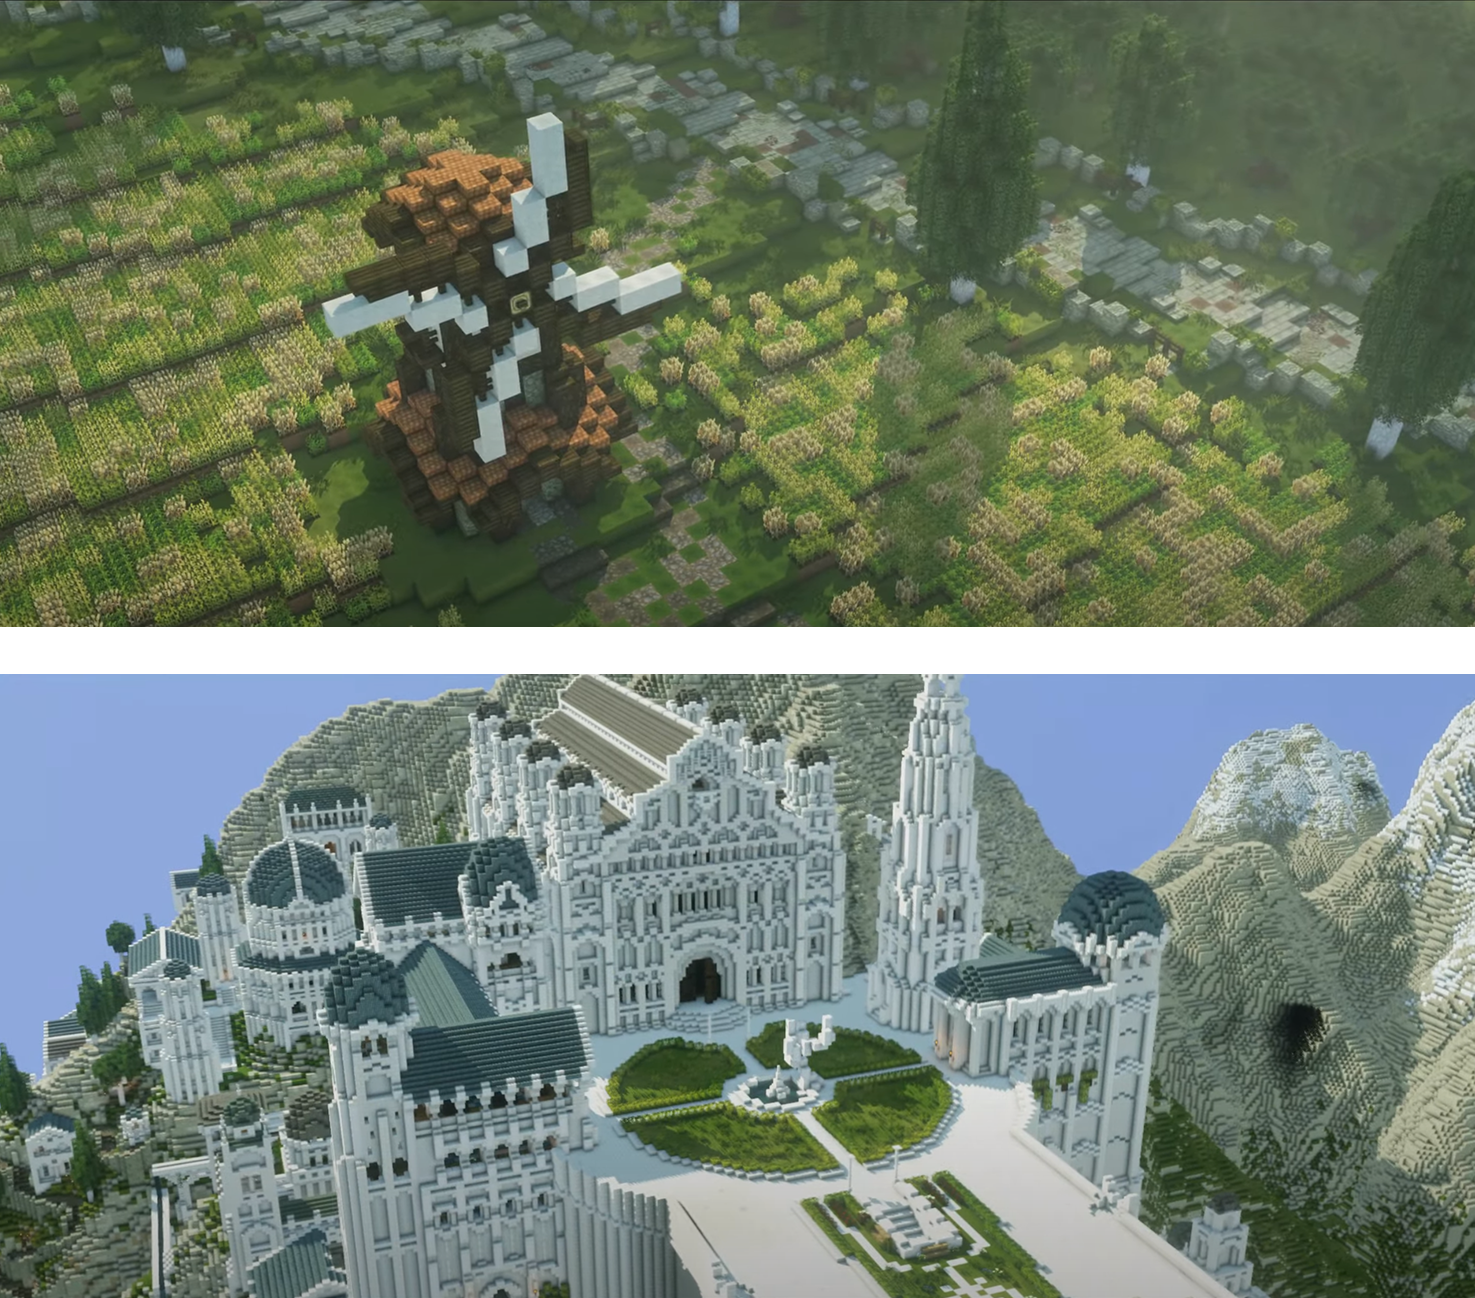
\includegraphics[width=0.7\textwidth]{images/minecraft.png}
        \caption{Voxelized representation of Minas Tirith in Minecraft \cite{minecraft2020minastirith}.\\A multitude of voxels can also represent high-resolution data, at a high computational memory cost (image below).
        }
        \label{fig:minecraft}
\end{figure}


This work focuses mainly on endeavors that work with voxel-based representations of 3D data. Similar to how 2D data can be represented in a 2D matrix, 3D data can be represented as a regular grid in the three-dimensional space \cite{ahmed2018survey}, where each cell or region contains information about the objects that are inside of it, if it is occupied or not, etc. These regions in a 3D grid are called voxels. Figure \ref{fig:minecraft} visualizes a video game called Minecraft, where the low resolution can be seen as voxels, even though the rendering engine used is not voxel-based. The main disadvantage of using voxels in high-resolution data is the amount of unnecessary memory storage required. However, one can leverage sparse voxel octrees (SVO) to down-sampling 3D scenes and navigate a simplified version of the environments. Accordingly, this thesis work leverages SVOs and low-resolution voxels (occupancy grids) to explore 3D simplified environments and and scan objects. The motivation for this is two-fold: first, as described by \cite{mcgraw2020high}, SVOs provide a huge reduction of memory requirements for most scenes, since empty space is not explicitly stored. Second, voxels describe the 3D structure of objects in a low-resolution fashion, and they can be used as extrinsic rewards to motivate a learning agent to explore thorough trajectories around objects. These trajectories then serve the purpose of exploring objects from multiple angles. % e biggest disadvantage is for rendering purposes, but this thesis uses
For further discussion on different representations of 3D data, one can refer to these outstanding surveys \cite{ahmed2018survey, ioannidou2017deep}. 


\begin{figure}[!ht]
        \centering
        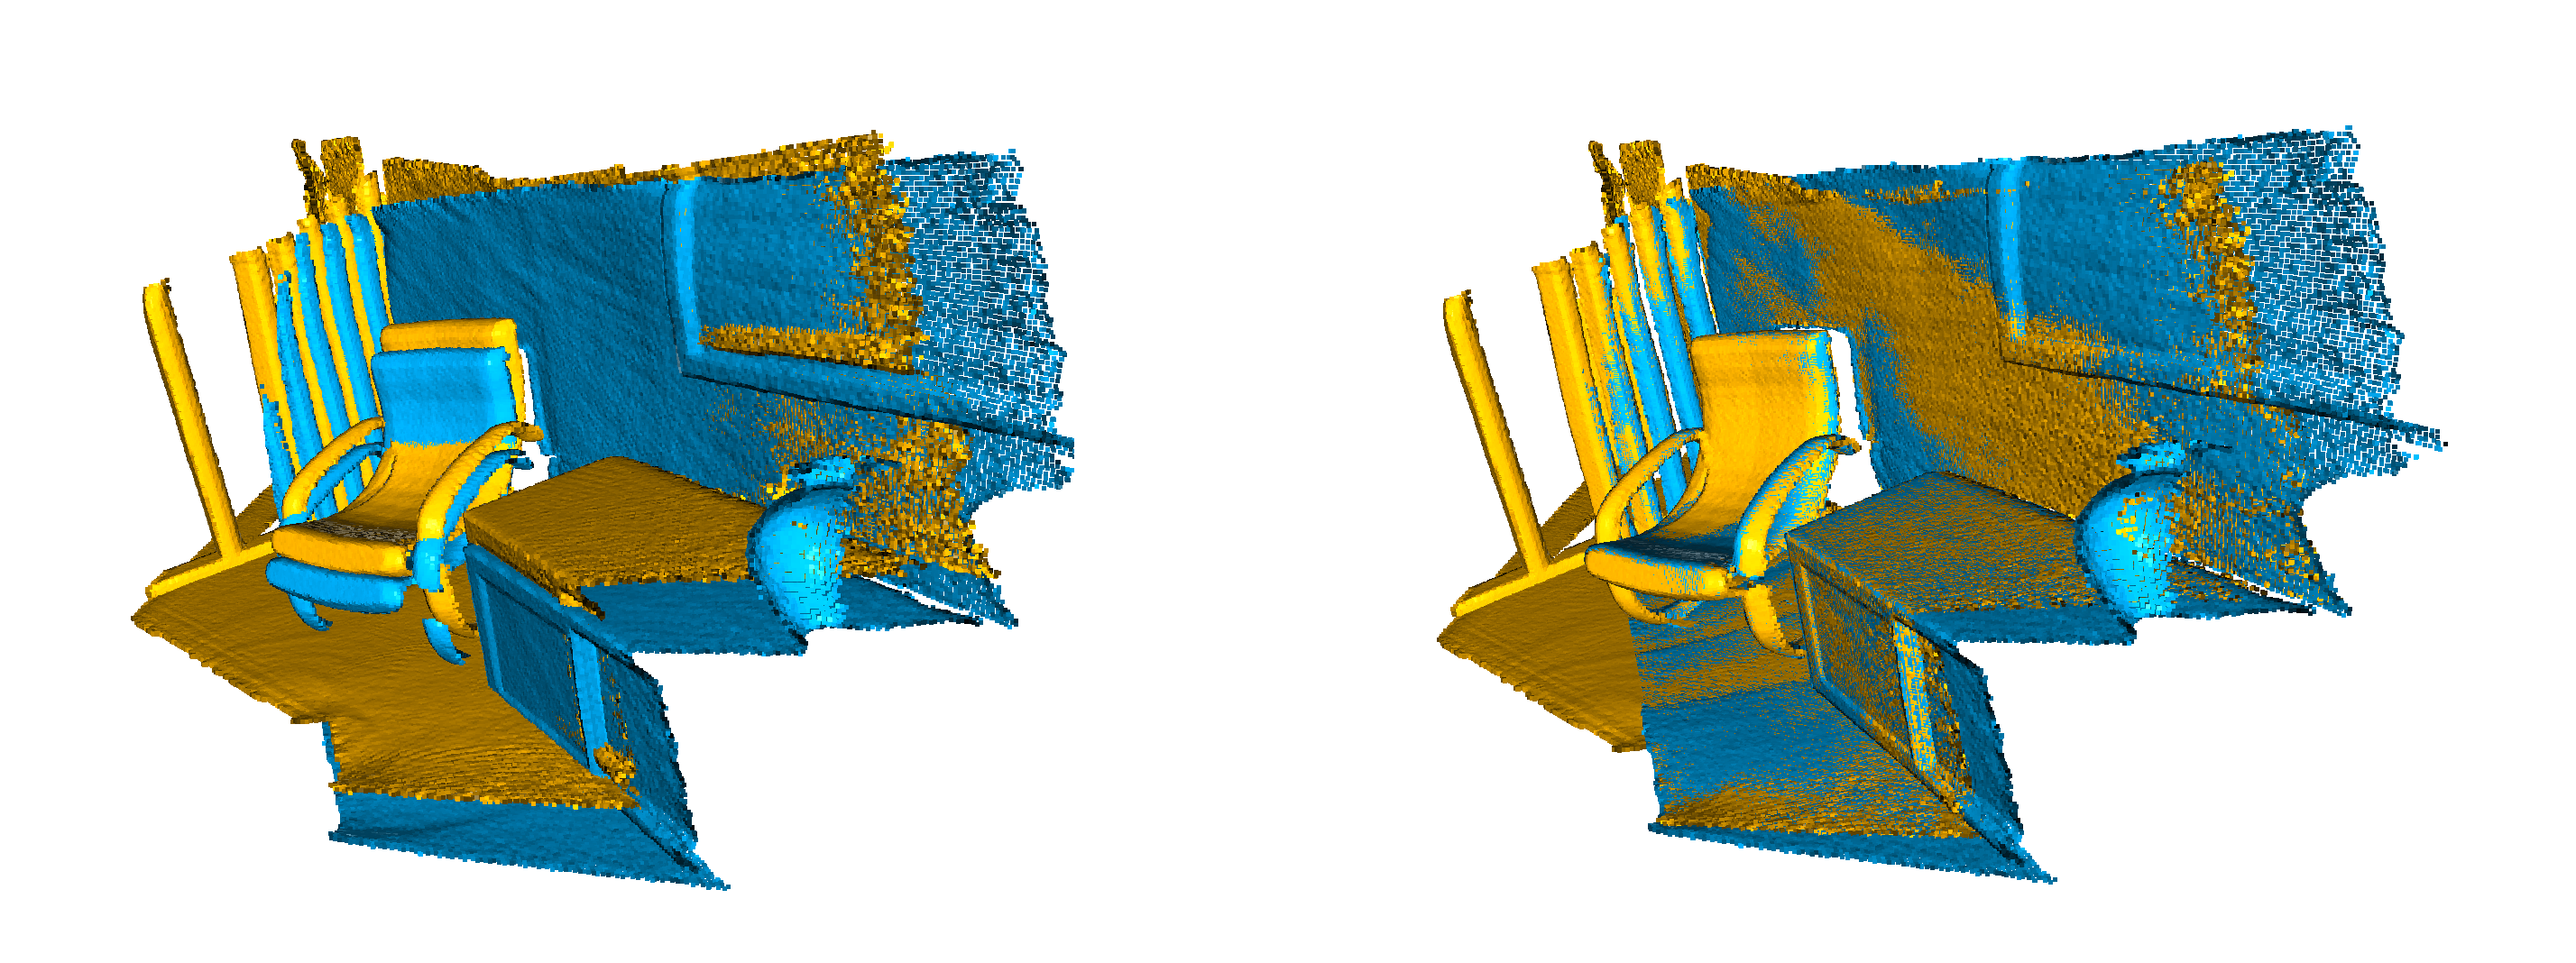
\includegraphics[width=0.8\textwidth]{images/icpalgorithm.png}
        \caption{Two input point clouds (left). Result after running the ICP Algorithm until convergence (right) \cite{open3D2021icp}.
        }
        \label{fig:icpalgorithm}
\end{figure}


Given an RGBD image, the process of generating a voxel grid from a triangle mesh is called voxelization \cite{open3D2021voxelization}. A voxel contains per default a "0" in the space it encloses. A "1" is assigned if the voxel is intersected with a triangle. However, one must obtain a point cloud beforehand from the RGBD data sent by a camera. Many works \cite{jia2019new, huang2021comprehensive} occupy themselves with point clouds from RGBD data, point cloud registration and the problem of outlier filtering when matching the RGB channel and the depth channel. Outlier filtering is required given that the alignment between the two channels can suffer from varying lighting conditions, reflective characteristics and particular sensor attributes. The further alignment in point cloud registration must also take into account a global world model when merging two point clouds together. Figure \ref{fig:icpalgorithm} displays the ICP algorithm \cite{open3D2021icp} for matching two point clouds together. Ultimately, a point cloud can then be voxelized or down-sampled to voxels for further processing \cite{open3D2021pointcloud}.


% Moreover, for a detailed pipeline on how to go from point clouds to voxels, see Appendix \ref{}



% \subsection{From Point Clouds to Voxels}\label{chap:2:pc-segmentation}
% This work aims to contribute to research on exploratory techniques using reinforcement learning.

% - what are images
% https://web.stanford.edu/class/cs101/image-1-introduction.html
% - what are DEPTH images
% http://cs231n.stanford.edu/reports/2016/pdfs/407_Report.pdf
% http://stanford.edu/class/ee367/Winter2020/report/lee_hong_lee_report.pdf

% - what are point clouds
% https://www.navvis.com/blog/everything-you-need-to-know-about-point-clouds-navvis


% - what are voxels
% https://en.wikipedia.org/wiki/Voxel
% % https://blog.spatial.com/the-main-benefits-and-disadvantages-of-voxel-modeling
% https://www.gamersnexus.net/gg/762-voxels-vs-vertexes-in-games

% \textbf{Limitations of Voxels.}

% \textbf{Applications of Voxels.}


\section{Octrees}\label{chap2:octrees}


\begin{figure}[!ht]
        \centering
        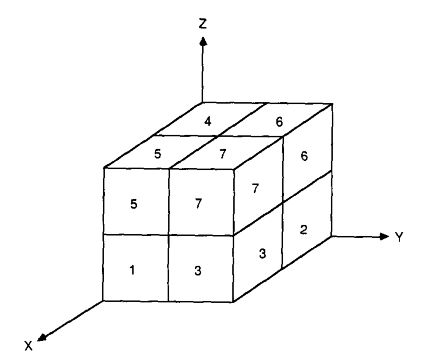
\includegraphics[width=0.4\textwidth]{images/octree.png}
        \caption{Labels of the octants of a cube (octant 0 is in the back and is not shown) \cite{chen1988survey}.
        }
        \label{fig:octree}
\end{figure}


% \textbf{Definition of Octrees. } 
The octree encoding uses a hierarchical tree data structure, where analog to quadtrees, each node can have up to eight children  \cite{meagher1980octree}. Octrees are used to model 3D spaces, since they allow the representation of a cubical region as shown in Figure \ref{fig:octree}. Whereas the root node represents the entire space, the rest of the octree is populated by the recursive subdivision of the 3D space into eight octants as shown in Figure \ref{fig:octree-vs-voxel}. Once the maximum resolution has been reached, nodes represent the leaves of the octree. Leaves in a node that have the same attributes can be reduced to a node by a process called condensation.
% ref here https://www.cg.tuwien.ac.at/studentwork/VisFoSe98/eder/octree.htm
Consequently, leaf nodes can be "point nodes" or "empty nodes", and a node that contains leaves is called a "region node".
% ref https://iq.opengenus.org/octree/\textbf

Information represented in leaves can be boolean or non-boolean if one decides to store more information in the tree such as temperature, etc. Condensation, however, is not a trivial process in non-boolean leaves. Finally, the implementation of octrees can be pointer-based or array-based. The pointer-based approach references child nodes as they are occupied by an object and are memory efficient. Array-based octrees define a priori all possible children in the hierarchy of the octree, making addressing of any node possible at the cost of memory.

 The resolution of the 3D space represented through an octree can be given as 2\textsuperscript{n}, and it is the octree's length space. The resulting volume enclosed by the octree consists of then $2\textsuperscript{n}\times2\textsuperscript{n}\times2\textsuperscript{n}$ octants. 
% Unit cubes can have values of 0 or 1 depending on the existence of objects inside of them.
% T
% When the maximum resolution is 
% There are different types of octrees, according to how the space is


% The octree space is usually modeled as a cubical region consisting of 2\^n x 2\^n x 2\^n 
% unit cubes, where n is the resolution parameter and 2\^n is the length of the octree 
% space. Each unit cube has value 0 or 1, depending on whether it is outside or inside
% the objects. 

% The octree representation of the objects is obtained by recursively
% subdividing the cubic space into octants.

% The results of the recursive subdivision process is represented by a tree of degree 
% 8 whose nodes are either leaves or have eight children. Thus, the tree is called an
% octree. Each node of the tree is given the same label as that assigned to its 
% corresponding o&ant. The root node of the resulting tree represents the entire space.

% Each node in an octree subdivides the space it represents into eight octants. 

% In a point region (PR) octree, the node stores an explicit three-dimensional point, which is the "center" of the subdivision for that node; the point defines one of the corners for each of the eight children. 
% In a matrix based (MX) octree, the subdivision point is implicitly the center of the space the node represents. 

% The root node of a PR octree can represent infinite space; 
% the root node of an MX octree must represent a finite bounded space so that the implicit centers are well-defined. 
% Note that Octrees are not the same as k-d trees: k-d trees split along a dimension and octrees split around a point. Also k-d trees are always binary, which is not the case for octrees.

% Less significant bits are sometimes ignored to reduce the tree size.
% The algorithm is highly memory efficient because the tree's size can be limited


% Three types of nodes are used in octree:

% Point node: Used to represent of a point. Is always a leaf node.
% Empty node: Used as a leaf node to represent that no point exists in the region it represent.
% Region node: This is always an internal node. It is used to represent a 3D region or a cuboid.


\begin{figure}[!ht]
        \centering
        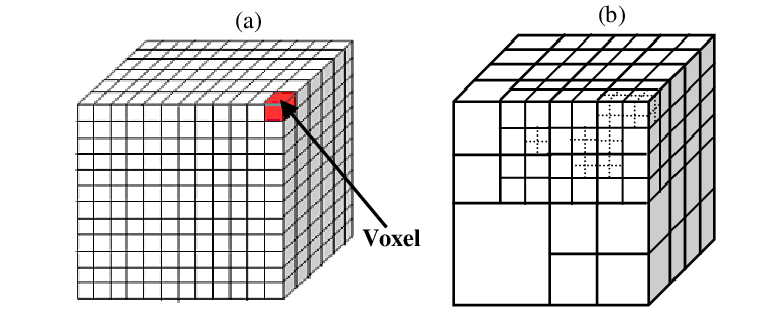
\includegraphics[width=0.7\textwidth]{images/voxelgridvsoctree.png}
        \caption{(a) Voxel grid (b) Octree representation \cite{saaidi2014multi}.
        }
        \label{fig:octree-vs-voxel}
\end{figure}


It is worth clarifying that the difference between a voxel grid and an octree is that a voxel grid is a fixed-resolution representation of 3D data, whereas the octree is multiresolution. When using in a rendering engine, octree rendering methods can load areas with higher resolution as one navigates the environment while keeping the other areas unloaded and preserving memory efficiency. A voxelgrid, in contrast, would always keep the same fixed resolution as one zooms in and out a render. Figure \ref{fig:octree-vs-voxel} aims to visualize the differences between an octree and a voxelgrid. For information on the complex manipulation of octrees and implementations of the search and insertion operations, please refer to \textcite{opengenus2021octree, geeksforgeeks2021octree}.
% https://iq.opengenus.org/octree/
% https://www.geeksforgeeks.org/octree-insertion-and-searching/

% \textbf{Sparse Voxel Octrees.}
% SVO is basically an octree, which holds only the mesh values (i.e. it is sparse) and only cubes (i.e. it is voxel, since general octree can hold points or triangles). I.e. SVO will hold only the visible cubes in minecraft, while all the invisible (not digged to yet) cubes are simply absent, resulting in a very efficient culling. Given that it is octree, we can use efficient O(log2(n)) search to check is that cube is visible to the player, compared to the usual grid raymarching, going over all the cells in line. Although the usual grid raymarching can still be speedup with signed distance field values inside empty grid cells. The O(log2(n)) per ray makes it fast enough for raycasting implementaton. But generally it used only as alternative to polygons, when you need to stream very detailed static models from the secondary storage or over the network, since animating voxel meshes is a very non-trivial subject, although it apparently can be done with signed distance fields, but it will be a bit slower than triangles. TLDR: SVOs are a way to render very large static meshes, that cant be fit into video memory and have to reside on disk drive to be preloaded on demand at the desired level of detail.

\textbf{Applications of Octrees.}
Octree's main application is using it as an acceleration structure given that memory and inference times increase cubically as the size of the 3D data increases. 
First, they excell as sparse data structures where empty regions consume little to no memory \cite{laine2010efficient}.
Second, in situations where meshes are too big for the available hardware, they allow efficient scaling through loading of 3D models at lower resolutions. 
Third, their efficient $O(log_{2}n)$ search queries when verifying the visibility of a cube make them an efficient data structure for high-quality ray casting of static scenes \cite{gobbetti2008single}.

Concretely, as proven by \textcite{elseberg2013one}, "octrees are well suited for storing large point cloud data, as it is a lossless compression, which reduces the size of a point cloud by a factor of roughly two and comes with a fast indexing". It is important to repeat and highlight that \textit{lossless compression} through octrees can be accelerated by a factor of two. To further support our claim of using octrees for exploration with a numeric example: one of the three datasets used by \textcite{elseberg2013one}, the \textit{Bunker Valentin} point cloud, has a file size of 665.7 MB in .txt format. Using octrees with lossless compression the file size goes down to 172.1 MB. Furthermore, using a leaf size node of 5.45 cm, the file size goes down to 14.93 MB.

The efficient representation of high-resolution 3D models using octrees in comparison to polygon-based methods has been further studied in a multitude of other works such as fast collision detection in models of over 25M polygons \cite{melero2019fast}, solar radiation \cite{liang2017sparse}, voxelized full-waveform airborne LIDAR data \cite{miltiadou2021comparative}, volume rendering methods \cite{knoll2006survey}, adaptive resolution SLAM \cite{vespa2019adaptive}, etc. In terms of limitations, octree-based techniques are not straight-forward since octrees are difficult to implement and manipulate. Moreover, operations on octrees in dynamic scenes where nodes need to be continuously recalculated are not efficient. This thesis limits itself to the usage of sparse boolean octrees as a mapping structure for a 3D scene where newly discovered nodes provide an intrinsic reward to the agent. Hence, the limitations of octrees are disregarded.



% Octree ray casting/tracing is just the act of raytacing, but using an octree as an acceleration structure rather than nothing or a uniform grid (like how traditional voxels are stored).
% Some advantages of using an octree is that A) ray collision queries can be accelerated by them, and B) octrees, and particularly sparse octrees, can make empty/air regions consume little or no storage.

% if your game uses raytracing, the graphics performance would be better using this data structure. In addition, octrees can reduce the memory footprint of large voxel scenes when there are lots of empty areas.
% https://www.reddit.com/r/VoxelGameDev/comments/ioe7wc/advantages_of_advanced_voxel_rendering_techniques/
% Advantages:
% Can represent crazy amount of detail as voxels that would be impossible with a polygon engine. With polygons, you need to LOD aggressively to keep things managable, here you can show intricate detail quite far away.
% Many basic rendering effects are very simple. You can have high quality shadows on everything with just a few lines of code, whereas managing shadow maps for polygon rendering efficiently is really hard.
% Modifying the world during gameplay probably easier than with polygons.
% Modern hardware is ready for it. I can render basic worlds represented with 36 trillion voxels at 4K in 60fps.. on a 1080Ti.
% Easy to scale. Doesn't run fast enough? render natively at a lower res.
% You get a "unique look" for your game, for free. Good to have nowadays.

% \textbf{Limitations of Octrees.}


% An obvious con of using this is that it can be harder to code than more basic solutions. There are likely other cons, but I don't want to speak outside my realm of knowledge here.

% I don't know which paper is "optimal", but I would search on Google scholar "efficient sparse voxel octrees" and look at some of the papers. Their implementation is brutal I hear, but the papers explain what is happening.

% Disadvantages:

% Though you do not strictly need LOD, dealing with aliasing effects if you don't do LOD. So you'll want the ray to stop at a certain size voxel. Use TAA if you can, its best at fixing the typical aliasing you get from ray-tracing.

% It's hard to efficiently have some rendering effects for some surfaces and not others. Your renderer works better the more uniform it is.

% Every extra ray costs a lot. I do a primary ray and a shadow ray, and a reflection ray would slow things down quite a bit.

% Not easy to do dynamic or animated objects. Again, everything has to be part of the same ray-cast to be efficient, so fastest would be to have your moving objects be part of the world structure somehow. Making them free-floating means you have to trace the world octree AND a model AABB tree or something for every ray, probably cutting your performance in half or worse. Or you could render models using polygons, and have them look funny when models and the world don't shadow each other correctly etc.

% Probably not great still on low end laptops or mobile hardware, even with the res scaled way down.

% You best enjoy writing your own rendering engines because EVERYTHING is going to be custom, and different from existing engines.

%  going into the 3d world
% point cloud segmentation, point cloud registration, scene understanding, and reinforcement learning 
\section{Scene Understanding}\label{chap2:scene-understanding}
% \lipsum[1-3]
% the same way that iphones rose, smart robots will rise.
% As algorithms and technologies continue to improve over the years, we have witnessed the rise of smartphones, smart homes and now smart offices. 

In their 2020 Hype Cycle for Artificial Intelligence, Gartner projects smart robots to be at their peak of expectations in about 2 to 5 years. This projection goes hand-in-hand with another projection in the same hype cycle. Gartner projects that computer vision will be on the slope of enlightenment around the same period. This is where the experts predict computer vision will enable applications to exploit another input stream: vision. The same way that computers and embedded systems are able to interpret audio and text input from sensors, keyboards, microphones, etc., systems will have access to vision to perform a variety of tasks. 
% n will enable systems to leverage vision for a variety of tasks. 
As \textcite{singh2018fotonnet} describes, "the ability for robots and computers to see and understand the environment is becoming a burgeoning field, needed in autonomous vehicles, augmented reality, drones, facial recognition, and robotic helpers". Since the rise of the CNN \cite{krizhevsky2017imagenet} deep learning based methods for image classification have reached state of the art performance for 2D detection.
% Object localization and segmentation are extensions to the image classification problem, which .
% which current 2D methods can now tackle. 

% In this work the focus is one of the current challenges for computer vision: 3D object recognition. As of today

% available 2D information, new geometric features, etc. 
% Even though 3D labeled data sets are scarce \cite{singh}, this is slowly changing \cite{google}\cite{3ddataset}. Likewise, 3D-depth sensors are not widely available as of today \ref{singh}, but this is slowly changing \ref{cheap-3d-sensors-phone}. 
% to 3D-image sensors in phone 
% due to the growing availability of public large data sets. low-cost 3D image sensors,  in the development phase, due in great part to a lack of publicly available large data sets. 

% \textbf{Definition of Scene Understanding.}
\begin{figure}[!ht]
        \centering
        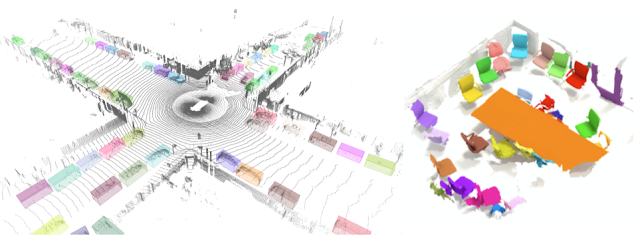
\includegraphics[width=0.9\textwidth]{images/sceneU01.png}
        \caption{3D object detection (left) and 3D instance segmentation (right) using Tensorflow 3D as found in \cite{najibi2020dops}.
        }
        \label{fig:sceneU01}
\end{figure}


The visible growth over the past few years of 3D sensors in our day-to-day surroundings (LIDAR, depth cameras, radar) comes hand-in-hand with the requirement for efficient and accurate machine-learning-powered scene understanding methods that can process the data coming from these sensors. Suitable example applications are self-driving cars and robots where they need a sense of embodiment to interpret their environments and navigate around them or augmented reality experiences. Consequently, even though research in computer vision has been recently pushing the state-of-the-art techniques in 3D object detection, much remains to be done to improve the workflow and research of techniques using 3D data. Libraries like Tensorflow3D \cite{najibi2020dops}, Pytorch3D \cite{ravi2020pytorch3d}, Torch-Points3D \cite{tp3d}, Pytorch Geometric \cite{Fey/Lenssen/2019}, etc., aim to make deep learning models and dataset processing tools available to developers and researchers. Some of the main research areas include: 3D semantic segmentation, 3D object shape prediction, point cloud registration and point cloud densification.

% This is a framework for running common deep learning models for point cloud analysis tasks against classic benchmark. It heavily relies on Pytorch Geometric and Facebook Hydra.

% The framework allows lean and yet complex model to be built with minimum effort and great reproducibility. It also provide a high level API to democratize deep learning on pointclouds. See our paper at 3DV for an overview of the framework capacities and benchmarks of state-of-the-art networks.



% https://ai.googleblog.com/2021/02/3d-scene-understanding-with-tensorflow.html
% add picture from TF
Given the inherent sparse nature of 3D data in our surroundings, denoted as open space, appropriate data structures and algorithms for efficient memory and inference operations are required. Accordingly, sparse convolutional models with pooling operations are seen in the core backbones of most state-of-the-art methods used in outdoor autonomous driving and indoor benchmarks, such as Waymo, NuScenes and ScanNet \cite{najibi2020dops}.
Tensorflow, for example, uses the 3D submanifold sparse U-net architecture to extract both coarse and fine features from voxels. This network, as shown in Figure \ref{fig:u-net}, consists of three components: an encoder, a bottleneck and a decoder. A set of prediction heads can then be added according to the task at hand. Implementations involving sparse convolutions combined with CUDA techniques show improvements of up to 20x with respect to previous implementations \cite{najibi2020dops}.

% \begin{figure}[!ht]
%         \centering
%         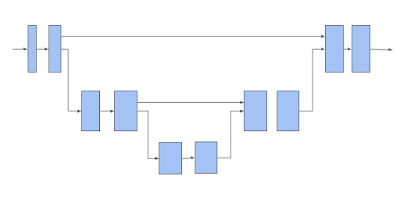
\includegraphics[width=0.65\textwidth]{images/u-net.png}
%         \caption{ A 3D sparse voxel U-Net architecture using submanifold sparse convolutions (horizontal arrows) and submanifold sparse pooling (arrows downward) operations \cite{tf}.
%         }
%         \label{fig:u-net}
% \end{figure}


% make a couple sentences
% 3D Sparse Convolutional Network
% The 3D data captured by sensors often consists of a scene that contains a set of objects of interest (e.g. cars, pedestrians, etc.) surrounded mostly by open space, which is of limited (or no) interest. As such, 3D data is inherently sparse.

% Sparse convolutional models are core to the state-of-the-art methods applied in most outdoor self-driving (e.g. Waymo, NuScenes) and indoor benchmarks (e.g. ScanNet).In such an environment, standard implementation of convolutions would be computationally intensive and consume a large amount of memory. 

% So, in TF 3D we use submanifold sparse convolution and pooling operations, which are designed to process 3D sparse data more efficiently. 

% We also use various CUDA techniques to speed up Experiments on the Waymo Open dataset shows that this implementation is around 20x faster than a well-designed implementation with pre-existing TensorFlow operations.

% TF 3D then uses the 3D submanifold sparse U-Net architecture to extract a feature for each voxel. The U-Net architecture has proven to be effective by letting the network extract both coarse and fine features and combining them to make the predictions.
% The U-Net network consists of three modules, an encoder, a bottleneck, and a decoder, each of which consists of a number of sparse convolution blocks with possible pooling or un-pooling operations.


% A 3D sparse voxel U-Net architecture. Note that a horizontal arrow takes in the voxel features and applies a submanifold sparse convolution to it. An arrow that is moving down performs a submanifold sparse pooling. An arrow that is moving up will gather back the pooled features, concatenate them with the features coming from the horizontal arrow, and perform a submanifold sparse convolution on the concatenated features.


% The sparse convolutional network described above is the backbone for the 3D scene understanding pipelines that are offered in TF 3D. Each of the models described below uses this backbone network to extract features for the sparse voxels, and then adds one or multiple additional prediction heads to infer the task of interest. 
% The user can configure the U-Net network by changing the number of encoder / decoder layers and the number of convolutions in each layer, and by modifying the convolution filter sizes, which enables a wide range of speed / accuracy tradeoffs to be explored through the different backbone configurations

% discussion future work, add photo of encoder
% In our recent paper, “DOPS: Learning to Detect 3D Objects and Predict their 3D Shapes”, we describe in detail the single-stage weakly supervised learning algorithm used for object detection in TF 3D. In addition, in a follow up work, we extended the 3D object detection model to leverage temporal information by proposing a sparse LSTM-based multi-frame model. We go on to show that this temporal model outperforms the frame-by-frame approach by 7.5% in the Waymo Open dataset.


\textbf{Applications of 3D Scene Understanding.}
Scene understanding techniques have been seen in a multitude of tasks, such as: rendering textured meshes or point clouds, camera position estimation, fitting meshes with textures, pose estimation, point cloud completion, and point cloud registration \cite{najibi2020dops, ravi2020pytorch3d}. A great effort has gone particularly into:
\begin{itemize}
    \item Semantic segmentation, where models predict per-voxel semantic scores using one output head, which are then mapped and used to label 3D points \cite{najibi2020dops, hackel2017semantic3d, qi2017pointnet, qi2017pointnet++}.
    \item Instance segmentation, where models group voxels that belong to the same object together using a per-voxel instance embedding vector and then predict a semantic score per-voxel. When the input consists of a point cloud instead of an image, methods using sparse 3D convolutions are preferred \cite{najibi2020dops, jiang2020pointgroup}.
    \item Object detection, where models uses box prediction and classification losses to predict per-voxel semantic scores, size, rotation matrices, and center, which are then reduced to accurate box proposals during inference time \cite{najibi2020dops, qi2019deep}. 
\end{itemize}

\textbf{Limitations of 3D Scene Understanding.}
% Scene Understanding Using Deep Neural Networks—Objects, Actions, and Events: A Review
As documented by \textcite{surendran2020scene}, the major drawbacks of current deep learning techniques include computational complexity and execution speed particular to each technique. Nevertheless, attaining high accuracy is one of the core challenges, especially in terms of distinguishing similar categories (selectivity) and in terms of robustness to rotations, scaling, translations and illumination changes (invariance).
One of the main causes for these symptoms in scene understanding research is the limited amount of publicly available 3D data sets \cite{han2019image}.
Research \cite{hackel2017semantic3d} highlights that the lack of rich 3D datasets is a major challenge in scene understanding research. For example, the Oakland dataset consists of less than 2 million labelled points, the NYU benchmark contains only indoor scenes and other data sets created using a 3D Velodyne LIDAR provide low point density meshes than those using a static scanner.
Another cause consists of the lack of accessibility for developers to hardware \cite{singh2018fotonnet} for 3D workflows. 

\begin{figure}[!ht]
        \centering
        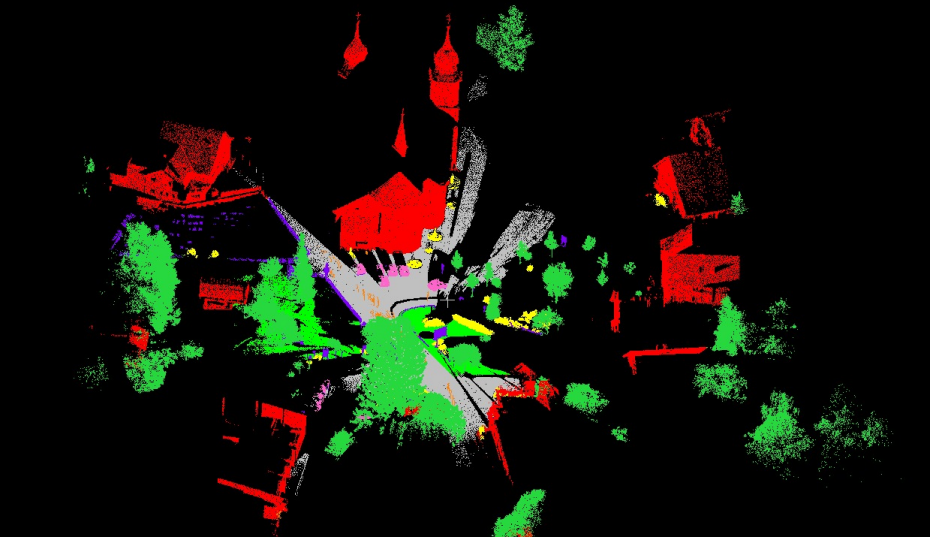
\includegraphics[width=0.7\textwidth]{images/sceneU02-hackel.png}
        \caption{Class labels example of Semantic3D \cite{hackel2017semantic3d}.
        }
        \label{fig:3Dsegsem-hackel}
\end{figure}


These two delaying factors are fortunately slowly changing: RGB-D data sets continue to be released to support the development of new algorithms. For example, the work by \textcite{hackel2017semantic3d} from ETH aids to the limited datasets problem by contributing with Semantic3D, the largest known labelled 3D point cloud data set of natural scenes, containing over 4 billion points. Another example is the MediaPipe data set released by Google in November of 2020 \cite{objectron2021dataset}. Moreover, accessibility to low-cost 3D sensors continues to increase: the newest smartphones, for example, are equipped with time-of-flight cameras, not only for photography but also extend their capabilities for AR applications and gaming \cite{tian2019occlusion}. Even though it is still not possible for any RGB-D data set to be as big as the ImageNet data set (∼5 million images), techniques continue to be developed to exploit geometric features and to utilize tools and concepts from 2D methods for 3D visual interpretation.

This thesis is motivated by the limitations present in the scene understanding field, and describes the promise of synthetic data in the following sections, which is then later exploited in the approach described in Chapter \ref{chap:3:title}. Similarly, given the limited amount of time and the extensive library of 3D methods, this work is constrained to 2D object detectors to define the concept of temporal uncertainty in a 3D scene, explained in the same chapter.
For more information on 2D object detectors, please refer to Appendix \ref{appendix:DL-for-vision}.

% https://ai.googleblog.com/2021/02/3d-scene-understanding-with-tensorflow.html
%  make one bullet point of each
% 3D Semantic Segmentation
% The 3D semantic segmentation model has only one output head for predicting the per-voxel semantic 

% 3D Instance Segmentation
% In 3D instance segmentation, in addition to predicting semantics, the goal is to group the voxels that belong to the same object together. The 3D instance segmentation algorithm used in TF 3D is based on our previous work on 2D image segmentation using deep metric learning. The model predicts a per-voxel instance embedding vector as well as a semantic score for each voxel. The instance embedding vectors map the voxels to an embedding space where voxels that correspond to the same object instance are close together, while those that correspond to different objects are far apart. In this case, the input is a point cloud instead of an image, and it uses a 3D sparse network instead of a 2D image network. At inference time, a greedy algorithm picks one instance seed at a time, and uses the distance between the voxel embeddings to group them into segments.

% 3D Object Detection
% The 3D object detection model predicts per-voxel size, center, and rotation matrices and the object semantic scores. At inference time, a box proposal mechanism is used to reduce the hundreds of thousands of per-voxel box predictions into a few accurate box proposals, and then at training time, box prediction and classification losses are applied to per-voxel predictions.
% We apply a Huber loss on the distance between predicted and the ground-truth box corners. 
% Since the function that estimates the box corners from its size, center and rotation matrix is differentiable, the loss will automatically propagate back to those predicted object properties. 3
% We use a dynamic box classification loss that classifies a box that strongly overlaps with the ground-truth as positive and classifies the non-overlapping boxes as negative.


% https://prs.igp.ethz.ch/research/current_projects/3D_scene_understanding.html

% 3D point cloud classification is an important task with applications in robotics, augmented reality and urban planning.
% Recent advances in Machine Learning and Computer Vision have proven that complex real-​world tasks require large training data sets for classifier training. 
% At the same time, until now there were no data sets for 3D point cloud classification which would be sufficiently rich in both object representations and number of labelled points. For example, the well-​known Oakland data set contains less than 2 million labelled points. Another popular data set, the NYU benchmark, provides only indoor scenes. Finally, both Sydney Urban Objects data set and the IQmulus & TerraMobilita Contest use a 3D Velodyne LIDAR mounted on a car which provides much lower point density than a static scanner. The same counts for the Vaihingen3D airborne benchmark.

% This benchmark closes the gap and provides the largest known labelled 3D point cloud data set of natural scenes with over 3 billion points in total. It also covers a range of diverse urban scenes: churches, streets, railroad tracks, squares, villages, soccer fields, castles to name just a few. The point clouds we provide are scanned statically with state-​of-the-art equipment and contain very fine details. Our goal is to help data-​demanding methods like deep neural nets to unleash their full power and to learn richer 3D representations than it was ever possible before.

% https://ai.googleblog.com/2021/02/3d-scene-understanding-with-tensorflow.html
% https://prs.igp.ethz.ch/research/current_projects/3D_scene_understanding.html
% https://arxiv.org/pdf/2103.06422.pdf
% https://ethz.ch/content/dam/ethz/special-interest/baug/igp/photogrammetry-remote-sensing-dam/documents/pdf/wojek12.pdf

% Along these lines, research from 2020, such as PointContrast \cite{xie2020pointcontrast} and OcCo \cite{wang2020pre} propose pre-training on ShapeNet \cite{chang2015shapenet} to leverage the information contained in point clouds for scene understanding and for reconstructing occluded point clouds respectively. Figure \ref{fig:occo-results} illustrates the performance of OcCo pre-training  for completion of occluded point clouds.

% - some relevant works on PC
% https://prs.igp.ethz.ch/research/current_projects/registration-of-3dpoint-clouds-with-low-overlap.html
% https://prs.igp.ethz.ch/research/current_projects/geometric-deep-learning-for-point-cloud-processing.html
% https://ethz.ch/content/dam/ethz/special-interest/baug/igp/photogrammetry-remote-sensing-dam/documents/pdf/timo-jan-isprs2016.pdf

% \subsection{Understanding from Monocular Cameras}\label{chap:2:aa}


% \textbf{Monocular Videos.}
% Panoramic Visual SLAM Technology for Spherical Images

